%%
%\listfiles
%\documentclass[%
% reprint,%
%secnumarabic,%
% amssymb, amsmath,%
% aip,cha,%
%groupedaddress,%
%frontmatterverbose,
%]{revtex4-1}
\documentclass[twocolumn,amsmath,amssymb,showpacs,pre,nofootinbib,superscriptaddress]{revtex4-1} %,preprint,jcp

\bibstyle{apsrev}
%\usepackage{docs}%
\usepackage{bm}%
\usepackage{graphicx}
%\usepackage{subcaption}
\usepackage{tikz}
\usepackage{color}
\usepackage{xcolor}
\usepackage{physics}
\usepackage[colorlinks=true,linkcolor=blue]{hyperref}%
%\nofiles
\expandafter\ifx\csname package@font\endcsname\relax\else
 \expandafter\expandafter
 \expandafter\usepackage
 \expandafter\expandafter
 \expandafter{\csname package@font\endcsname}%
\fi
\hyphenation{title}
\newcommand{\JH}[1]{\textcolor{blue}{ JH: #1}}

\begin{document}

\definecolor{pyblue}{HTML}{1F77B4}
\definecolor{pyorange}{HTML}{FF7F0C}
\definecolor{pygreen}{HTML}{2CA02C}
\definecolor{pyred}{HTML}{D62728}
\newcommand*\Diff[1]{\mathop{}\!\mathrm{d^#1}}


%\title{Switchable substrates and thin film morphologies}
\title{Spatiotemporal varying contact angles and thin film morphologies}

\author{S. Zitz}
\email{s.zitz@fz-juelich.de}
 \affiliation{Helmholtz Institute Erlangen-N\"urnberg for Renewable Energy,\\
  Forschungszentrum J\"ulich,\\
  F\"urther Strasse 248, 90429 N\"urnberg, Germany}%
  \affiliation{Department of Chemical and Biological Engineering, Friedrich-Alexander-Universit\"at Erlangen-N\"urnberg, F\"{u}rther Stra{\ss}e 248, 90429 N\"{u}rnberg, Germany}
\author{A. Scagliarini}%
\email{andrea.scagliarini@cnr.it}
 \affiliation{Institute for Applied Mathematics "M. Picone" (IAC), \\
Consiglio Nazionale delle Ricerche (CNR),\\
Via dei Taurini 19, 00185 Rome, Italy}%
\affiliation{INFN, sezione Roma ``Tor Vergata'', via della Ricerca Scientifica 1, 00133 Rome, Italy}
\author{J. Harting}
\email{j.harting@fz-juelich.de}
 \affiliation{Helmholtz Institute Erlangen-N\"urnberg for Renewable Energy,\\
  Forschungszentrum J\"ulich,\\
  F\"urther Strasse 248, 90429 N\"urnberg, Germany}%
 \affiliation{Department of Chemical and Biological Engineering and Department of Physics, Friedrich-Alexander-Universit\"at Erlangen-N\"urnberg, F\"{u}rther Stra{\ss}e 248, 90429 N\"{u}rnberg, Germany}
\date{\today}

\begin{abstract}
We study the dynamics of an unstable thin film deposited on a ``switchable`` substrate.
The substrate is itself subject to a time varying function that affects the equilibrium contact angle $\theta_{\text{eq}}(\mathbf{x},t)$.
We show that in the case of vanishing time dependence the patterning drives the dewetting morphology and that all fluid is drained into regions of small $\theta_{\text{eq}}(\mathbf{x})$ and thus form droplets.
Interestingly enough with a time varying component to the pattern we are able to stop the droplet fragmentation and create pronounced ligament or rivulet morphologies.
We show that both the numbers of semistable rivulets as well as number of stable droplets can be controlled with the pattern wavelength ($\lambda$).
Finally we explain why the ligaments appear with a simple balance between capillary retraction and dynamic wetting.   
\end{abstract}

\maketitle

\newcommand{\ts}{\textsuperscript}
%\tableofcontents

\section{Introduction}\label{sec:intro}
Thin film flows and especially droplets are an phenomenon we experience in our every day life.
Being it the droplets condensed in the higher atmosphere and return to the ground as rain or the oil film in a pan during cooking. 
While this two examples are illustrative there are many industrial applications that build on thin film flows. 
Among them is the wetting of surfaces to reduce wear or put simply, lubrication~\cite{ReynoldsLubr, gross1980fluid, szeri2010fluid}. 
Coating surfaces to change their physio-chemical properties is another widely used application~\cite{DERYCK1998278, doi:10.1146/annurev.fluid.31.1.347, DASILVASOBRINHO19991204}.
On the other hand the need to control droplets is at the heart of many printing processes~\cite{singh2010inkjet, jo2009evaluation}.

More recently lab-on-a-chip devices have acquired much attention~\cite{C6LC00387G,Focke}, to work they require precise droplet or film flow on small scales~\cite{stone2004engineering, darhuber2010planar}.
One possibility for precise control is the local wettability.
Light switchable substrates~\cite{WANG200718}, therefore substrates that change their wettability based on light illumination, open up a new way to program this devices. 
From a theoretical point of view the motion of the fluid can be computed using the thin film equation~\cite{RevModPhys.69.931, RevModPhys.81.1131, RevModPhys.81.739, ReynoldsLubr}
\begin{equation}\label{eq:thin_film}
    \partial_t h(\mathbf{x},t) = \nabla\cdot\left(M(h)\nabla p(\mathbf{x},t)\right),
\end{equation}
where $h(\mathbf{x},t)$ is a time and spatial varying film thickness, $M(h)$ is a mobility function and $p(\mathbf{x},t)$ is a pressure term that drives the flow. 
The function $M(h)$ contains information about the velocity boundary condition at $h=0$, using no-slip yields $M(h) = h^3/(3\mu)$.
More interesting however is the pressure function $p(\mathbf{x},t)$ as it allows to model the wettability of a given substrate.
We therefore introduce a time and spatial dependent contact angle to control the local wettability.

Spatial variations of the contact angle are long known and used in previous studies~\cite{PhysRevE.91.023013, Sommers_2006}, time dependency of the contact angle on the other hand is not as well studied~\cite{suman2006dynamics}. 
Switchable substrates are in fact a realization of a time dependent contact angle. 
Using both spatial as well as time dependent variations of the local contact angle leads to interesting phenomena, for example continuously sliding droplets as shown by Grawitter and Stark~\cite{D0SM02082F}.  
Our approach builds on the same idea but our method, see ref~\cite{PhysRevE.100.033313}, allows us to go beyond a single droplet and to simulate the full dewetting transition starting with a thin film and ending with droplets.
We use this to show that a time dependent component of the contact angle alter the dewetting morphology quite substantially.
In the limit of a small time dependency or slow evolution of the contact angle field we qualitatively reproduce the results from Grawitter and Stark, such sliding droplets.
Speeding up the evolution of the contact angle field introduces a morphological transition, which to the understanding of the authors have not been looked at so far.
Therefore the purpose of this manuscript is to increase the understanding of the dewetting process.
Highlighting the fact that a temporal and spatial variation of the contact angle leads to novel morphological structures.
Thus our finding offer a simple way to understand how time periodic switchable substrates could generate novel dewetting morphologies.

The manuscript is outlined as follows:
In section~\ref{sec:method} we discuss the numerical method we use to generate our results and introduce relevant scales.
We then present our results in section~\ref{sec:results}, where we discuss the impact of the time dependency on the contact angle and show that both stability as well as dewetting morphology is affected.
A short summary of our finding and a closing conclusion with outlook is given in section~\ref{sec:sum_conclu}.

\section{Method}\label{sec:method}
In this section we describe the lattice Boltzmann method (LBM) we use.
The LBM is a meso scale approach that builds on the Boltzmann equation to simulate fluid flows~\cite{krueger2017}. 
It is widely applied to many kinds of flow problems, among them are for instance multi phase and multi component flows~\cite{shan1993lattice,PhysRevE.73.047701}, flows through porous media~\cite{liu2016multiphase} and shallow water flows~\cite{Salmon:1999:0022-2402:503, zhou2004lattice, PhysRevE.65.036309}.
The model we use has been introduced in ref.~\cite{PhysRevE.100.033313} and builds upon a class of lattice Boltzmann models originally developed to study the shallow water equations~\cite{Salmon:1999:0022-2402:503, PhysRevE.65.036309}.

\subsection{Thin film lattice Boltzmann method}\label{subsec:LBM}
Since the model has been developed and tested in previous work, ref.~\cite{PhysRevE.100.033313}, we just outline the most important features.
The internal degrees of freedom of this method are the distributions functions $f_{\alpha}(\mathbf{x},t)$.
These distribution functions describe the movement of fictitious particles on a lattice, in this case on a $D2Q9$ lattice.
Meaning there are nine velocity components ($Q9$), directions in which a particle could move, for a simulation in two dimensions ($D2$).
The dynamics of the thin film and thus the evolution of the distribution functions is given by
\begin{equation}\label{eq:LBE}
    \begin{split}
        &f_{\alpha}(\mathbf{x}+\mathbf{c}^{({\alpha})}\Delta t,t+\Delta t) = \\
        &\left(1 - \frac{\Delta t}{\tau}\right) f_i(\mathbf{x},t) + \frac{\Delta t}{\tau} f_{\alpha}^{(eq)}(\mathbf{x},t) + \Delta t\mathcal{S}_{\alpha},
    \end{split}
\end{equation}
where the $\mathbf{c}^{({\alpha})}$ are the $Q$ discrete lattice velocities that can be computed according to
\begin{equation}\label{eq:speeds}
\mathbf{c}^{({\alpha})}  =
\left\{
\begin{array}{ll}
(0,0) & \alpha = 0 \\
\left[\cos{\frac{(\alpha-1)\pi}{4}}, \sin{\frac{(\alpha-1)\pi}{4}} \right] &  \alpha=1,3,5,7 \\
\sqrt{2}\left[\cos{\frac{(\alpha-1)\pi}{4}}, \sin{\frac{(\alpha-1)\pi}{4}} \right] & \alpha=2,4,6,8
\end{array}
\right.,
\end{equation}
and $w$ are being the corresponding weights
\begin{equation}
w_{\alpha}  =
\left\{
\begin{array}{ll}
\frac{4}{9} & \alpha = 0 \\
\frac{1}{9} &  \alpha=1,3,5,7 \\
\frac{1}{36} & \alpha=2,4,6,8
\end{array}
\right..
\end{equation}
The last term to the right $\mathcal{S}_{\alpha}$ is a (generalized) source term.
The concrete implementation of the forces depend on the source term as~\cite{https://doi.org/10.1002/fld.4726}
\begin{equation}\label{eq:source_term}
    \mathcal{S}_{\alpha} = \frac{3w_{\alpha}}{\mathbf{c}_{\alpha}^2}\mathbf{c}_{\alpha}\cdot\mathbf{F}.
\end{equation}
We are able to match thin film dynamics with the usage of a force term comprising of two main components,
\begin{equation}\label{eq:forcesum}
    \mathbf{F} = \mathbf{F}_{\mbox{\tiny{fric}}} + \mathbf{F}_{\mbox{\tiny{film}}}.
\end{equation}
The first being a friction force that includes a velocity boundary condition at the fluid substrate interface
\begin{equation}\label{eq:forcefric}
\mathbf{F}_{\mbox{\tiny{fric}}} = -\frac{6h\mu\mathbf{u}}{2h^2+6\delta h + 3\delta^2},
\end{equation}
where $\mu$ is the viscosity and $\delta$ is a socalled slip length~\cite{RevModPhys.69.931, PhysRevE.100.033313, PhysRevE.63.011208, munch_lubrication_2005}.
The film thickness $h$ is the zeroth moment of the distribution function $f_{\alpha}$, i.e. $h(\mathbf{x},t) = \sum_{\alpha}f_{\alpha}(\mathbf{x},t)$ see Eq.~(\ref{eq:LBE}). 
The second component is due to the film pressure $p_{\text{film}}$ and accounts for the minimization of the fluid vapor interface as well as for the wettability of the substrate,
\begin{equation}\label{eq:pressure_here}
    p_{\text{film}} = -\gamma (\Delta h - \Pi(h)),
\end{equation}
which results in the addition of the force $\mathbf{F}_{\mbox{\tiny{film}}}$
\begin{equation}\label{eq:forcefilm}
    \mathbf{F}_{\mbox{\tiny{film}}} = -\frac{h}{\rho_0}\nabla(p_{\text{film}}), 
\end{equation}
with $\gamma$ being the (constant) surface tension and $\rho_0$ being the fluids density, which is $\rho_0 = 1$ and will be dropped in the following. 
Here we model the interaction between solid substrate and film with a disjoining pressure term~\cite{RevModPhys.69.931, RevModPhys.81.1131, PhysRevE.63.011208},
\begin{equation}\label{eq:disjoinpressure}
    \Pi(h) = \kappa(\theta_{\text{eq.}})\left[\left(\frac{h_{\ast}}{h}\right)^n - \left(\frac{h_{\ast}}{h}\right)^m\right],
\end{equation}
with $n$ and $m$ being integer exponents, $h_{\ast}$ defines the minimum of the potential and  
\begin{equation}\label{eq:kappacontactangle}
    \kappa(\theta_{\text{eq.}}) = (1-\cos\theta_{\text{eq.}}) \frac{(n-1)(m-1)}{(n-m)h_{\ast}},
\end{equation}
which therefor allows us to tune the fluids contact angle.

\subsection{Linear stability and characteristic quantities}\label{subsec:charq}
For further insights concerning the early time dynamics of the unstable film we perform a linear stability analysis.
Thus we expand Eq.~(\ref{eq:thin_film}) in terms of a small perturbation $\delta h(\mathbf{x},t) = h(\mathbf{x},t) - h_0$ with $h_0$ being the initial mean thickness value at $t=0$.
Rearanging in terms up to first order in $\delta h$ yields
\begin{equation}\label{eq:linearstability_realspace}
    \partial_t \delta h = \frac{h_0^3}{3\mu}\nabla^2\Big(\Pi(\delta h) - \gamma \nabla^2 \delta h\Big).
\end{equation}
Under Fourier transformation of $\delta h$ 
\begin{equation}\label{eq:fouriertrans}
    \delta h(\mathbf{x},t) = \int(2\pi)^{-2}\delta \tilde{h}(\mathbf{q},t)e^{i\mathbf{q}\cdot\mathbf{x}}\Diff2\mathbf{q},
\end{equation}
and upon inserting this in Eq.~(\ref{eq:linearstability_realspace}) we get
\begin{equation}\label{eq:linearstab_fourier}
    \partial_t \delta \tilde{h}(\mathbf{q},t) = \omega(\mathbf{q})\delta\tilde{h}(\mathbf{q},t),
\end{equation}
with dispersion relation $\omega(q)$, 
\begin{equation}\label{eq:dispersion}
    \omega(\mathbf{q}) = \frac{1-(\frac{q^2}{q_0^2}-1)^2}{t_0}.
\end{equation}
Both, the maximum of the dispersion relation $q_0$ and therefore the characteristic time $t_0$, are specific to the substrate the film is deposited on and can be calculated using~\cite{PhysRevLett.99.114503}
\begin{equation}\label{eq:q0_and_t0}
    q_0^2 = \frac{1}{2}\frac{\partial \Pi(h)}{\partial h}\bigg\rvert_{h=h_0}, \qquad t_0 = \frac{3\mu}{\gamma h_0^3 q_0^4}.
\end{equation}

\subsection{Time and spatially varying contact angles $\theta(\mathbf{x},t)$}\label{subsec:theta}
To get a spatially varying contact angle $\theta(\mathbf{x},t)$ we make use of the underlying lattice and assign different values for $\theta$ to different grid points. 
From now on we drop the subscript \textit{eq.} for convenience, such $\theta = \theta_{\text{eq.}}$ unless otherwise stated.

We consider two different patterns and three wavelengths in this manuscript.
First being the sinusoidal pattern with wavelength $\lambda = L/i$ and wavenumbers $i=[1,2,3]$ which is given as
\begin{equation}\label{eq:sinetheta}
    \theta_1(x,y) = \theta_0 + \delta\theta\left[\sin\left(\frac{2\pi x}{\lambda}\right)\sin\left(\frac{2\pi y}{\lambda}\right)\right], 
\end{equation}
with $\theta_0 = 20^{\circ}$ and $\delta\theta=10^{\circ}$.
The second pattern is a triangle wave which accounts for a different kind of pattern gradient.
To the best of our knowledge contact angles can not be tuned precise enough to match a sinusoidal wave on the scales we are interested in.
Therefore we assume that a triangle wave with a linear gradient is more likely accessable in experiments, thus $\theta_2$ is given as
\begin{equation}\label{eq:triangle_wave}
\begin{split}
    \theta_2(x,y) &= \theta_0 + \\ &\frac{2\delta\theta}{\pi}\left[\sin^{-1}\left(\sin\left(\frac{2\pi x}{\lambda}\right)\right)\sin^{-1}\left(\sin\left(\frac{2\pi y}{\lambda}\right)\right)\right].
    \end{split}
\end{equation}

Both patterns create a contact angle distribution with values within the interval $[10^{\circ}, 30^{\circ}]$ and by definition they are time independent.
To have a time dependency we simply shift the pattern in a periodic manner, such that
\begin{equation}\label{eq:theta_shift}
    \theta(\mathbf{x},t+T) = \theta(\mathbf{x}-\mathbf{1}, t), 
\end{equation}
with $T$ being an arbitrary integer number of lattice Boltzmann time steps. 

Due to convenience we attribute a velocity to the pattern which is the shift distance divided by the stepping time
\begin{equation}\label{eq:pattern_speed}
    v_{\theta} = \frac{\sqrt{2}}{T}.
\end{equation}
Since this velocity as well as the choice of $T$ is arbitrary we define a characteristic velocity $v_0$ similar to Eqs.~(\ref{eq:q0_and_t0}) as
\begin{equation}\label{eq:normvel}
    v_0 = \frac{\lambda}{t_0(\theta)},
\end{equation}
where we use the wavelength $\lambda$ as a characteristic distance and $t_0(30^{\circ})$ as a characteristic time scale.
Important to note is that $t_0$ is sensitive to the contact angle, and decreases with increasing angle.

\subsection{Numerical system}
\begin{figure}
    \centering
    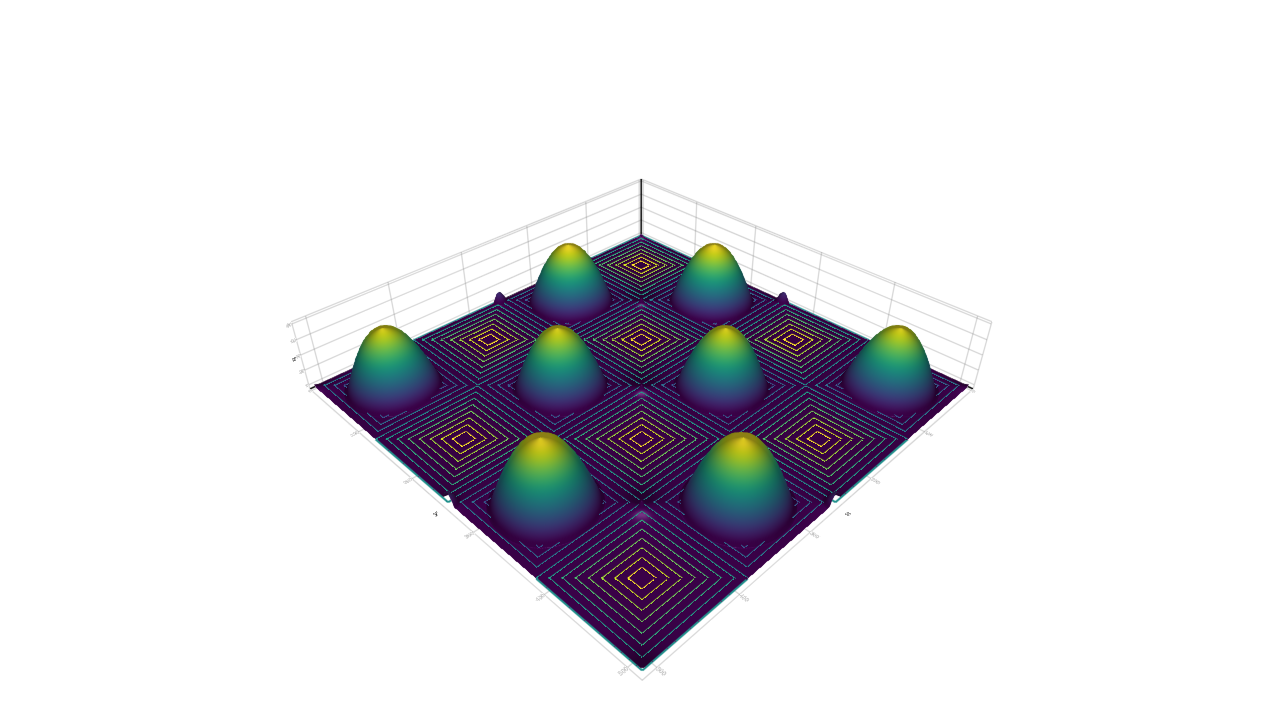
\includegraphics[width=0.45\textwidth]{Figures/makie_try2.png}
    \caption{Film thickness $h(\mathbf{x},t)$ at a stationary state. 
    The contact angle $\theta(\mathbf{x})$ is shown as contour.}
    \label{fig:handtheta}
\end{figure}
As outlined in Sec.~\ref{subsec:LBM} we simulate the evolution of the thin film with a lattice Boltzmann method.
For all our simulations we use periodic boundary conditions and a square of size $Lx = Ly = L = 512 \Delta x$ with $\Delta x = \Delta t = 1$.
The surface tension as well as the viscosity are constants and set to $\gamma = 0.01$ and $\nu|_{\rho_0=1} = \mu = 1/6$.
Having this value of $\mu$ leaves us with a relaxation time $\tau = 1$.
To regularize the contact line divergence~\cite{huh1971hydrodynamic} we use a precursor layer and a slip parameter $\delta = 1$. 
% With this choice of parameters we are almost able simulate a no-slip boundary condition.
As for our disjoining pressure potential, see Eq.~(\ref{eq:disjoinpressure}), we use the power pair $n=3, m=2$ and $h_{\ast} = 0.07$.
Inserting this quantities into Eq.~(\ref{eq:q0_and_t0}) with $h_0 = 1$ yields $q_0^2(30^{\circ}) \approx 1.68\cdot10^{-2}$ as well as $t_0(30^{\circ}) \approx 177000\Delta t$ which gives us a first glimpse into relevant length and time scales.

The initial condition of all our simulations is a film undulated with sinusoidal wave as
\begin{equation}\label{eq:hinitial}
    h(\mathbf{x},0) = h_0 \left[1 + \epsilon \left(\sin\left(\frac{2\pi x}{L}\right)\sin\left(\frac{2\pi y}{L}\right)\right)\right],
\end{equation}
with $\epsilon = 0.1$ and $h_0 = 1$.

We proceed as follows, first we simulate the dewetting on a given pattern either sinusoidal- or triangular with $\lambda \in \{L, L/2, L/3\}$ without a time dependency in $\theta$.
In Fig.~\ref{fig:handtheta} we show $h(\mathbf{x},t)$ as surface plot and $\theta_2(\mathbf{x})$ as contour plot for $v_{\theta} = 0, \lambda = L/2$ in late stages of dewetting.
Droplets form in regions of small contact angles while the regions of high contact angles dewet.
In subsequent simulations we iterate through $v_{\theta} \in [0.1, 1, 10]v_0$, see Eq.~(\ref{eq:normvel}) .  
% Based on $v_{\theta}$ we can modify the morphology of the dewetting film, in both the intermediate transition regime as well as the late time state.

\section{Results}\label{sec:results}
We now present our results and show how a time dependent wettability or pattern velocity alters the dynamics of a dewetting thin film.
In the following we address the growth of the initial perturbation $\delta h$ and the associated stability of the film.
Therefor we take a look at the rupture times and show that a pattern velocity $v_{\theta} > 0$ does have a stabilizing effect.

After rupture we discuss the morphological transitions the film undergoes.
Therefor the transition from a dewetting film to a droplet state.
This transition is heavily influenced by the concrete choice of $v_{\theta}$ and we observe a strong a alignment with the moving direction of the pattern.

Before we move to the case of $v_{\theta} > 0$ we like to draw a base line with simulation done with a stationary wettability profile.

\subsection{Stationary pattern}\label{subsec:no_vtheta}
Starting with Eq.~(\ref{eq:hinitial}) we have by definition an unstable film that will rupture.
This can be easily seen by the fact that the initial perturbation has the smallest possible wavenumber, $q(t=0)=1/L$.
Taking into account the addition of the wettability gradient we know that fluid will accumulate in regions of high surface energies or small contact angles and flow away from regions of high contact angle.
An illustrative results of this effect is shown in Fig.~\ref{fig:handtheta}, where all droplets are present in a region of small contact angles.

\begin{figure}
    \centering
    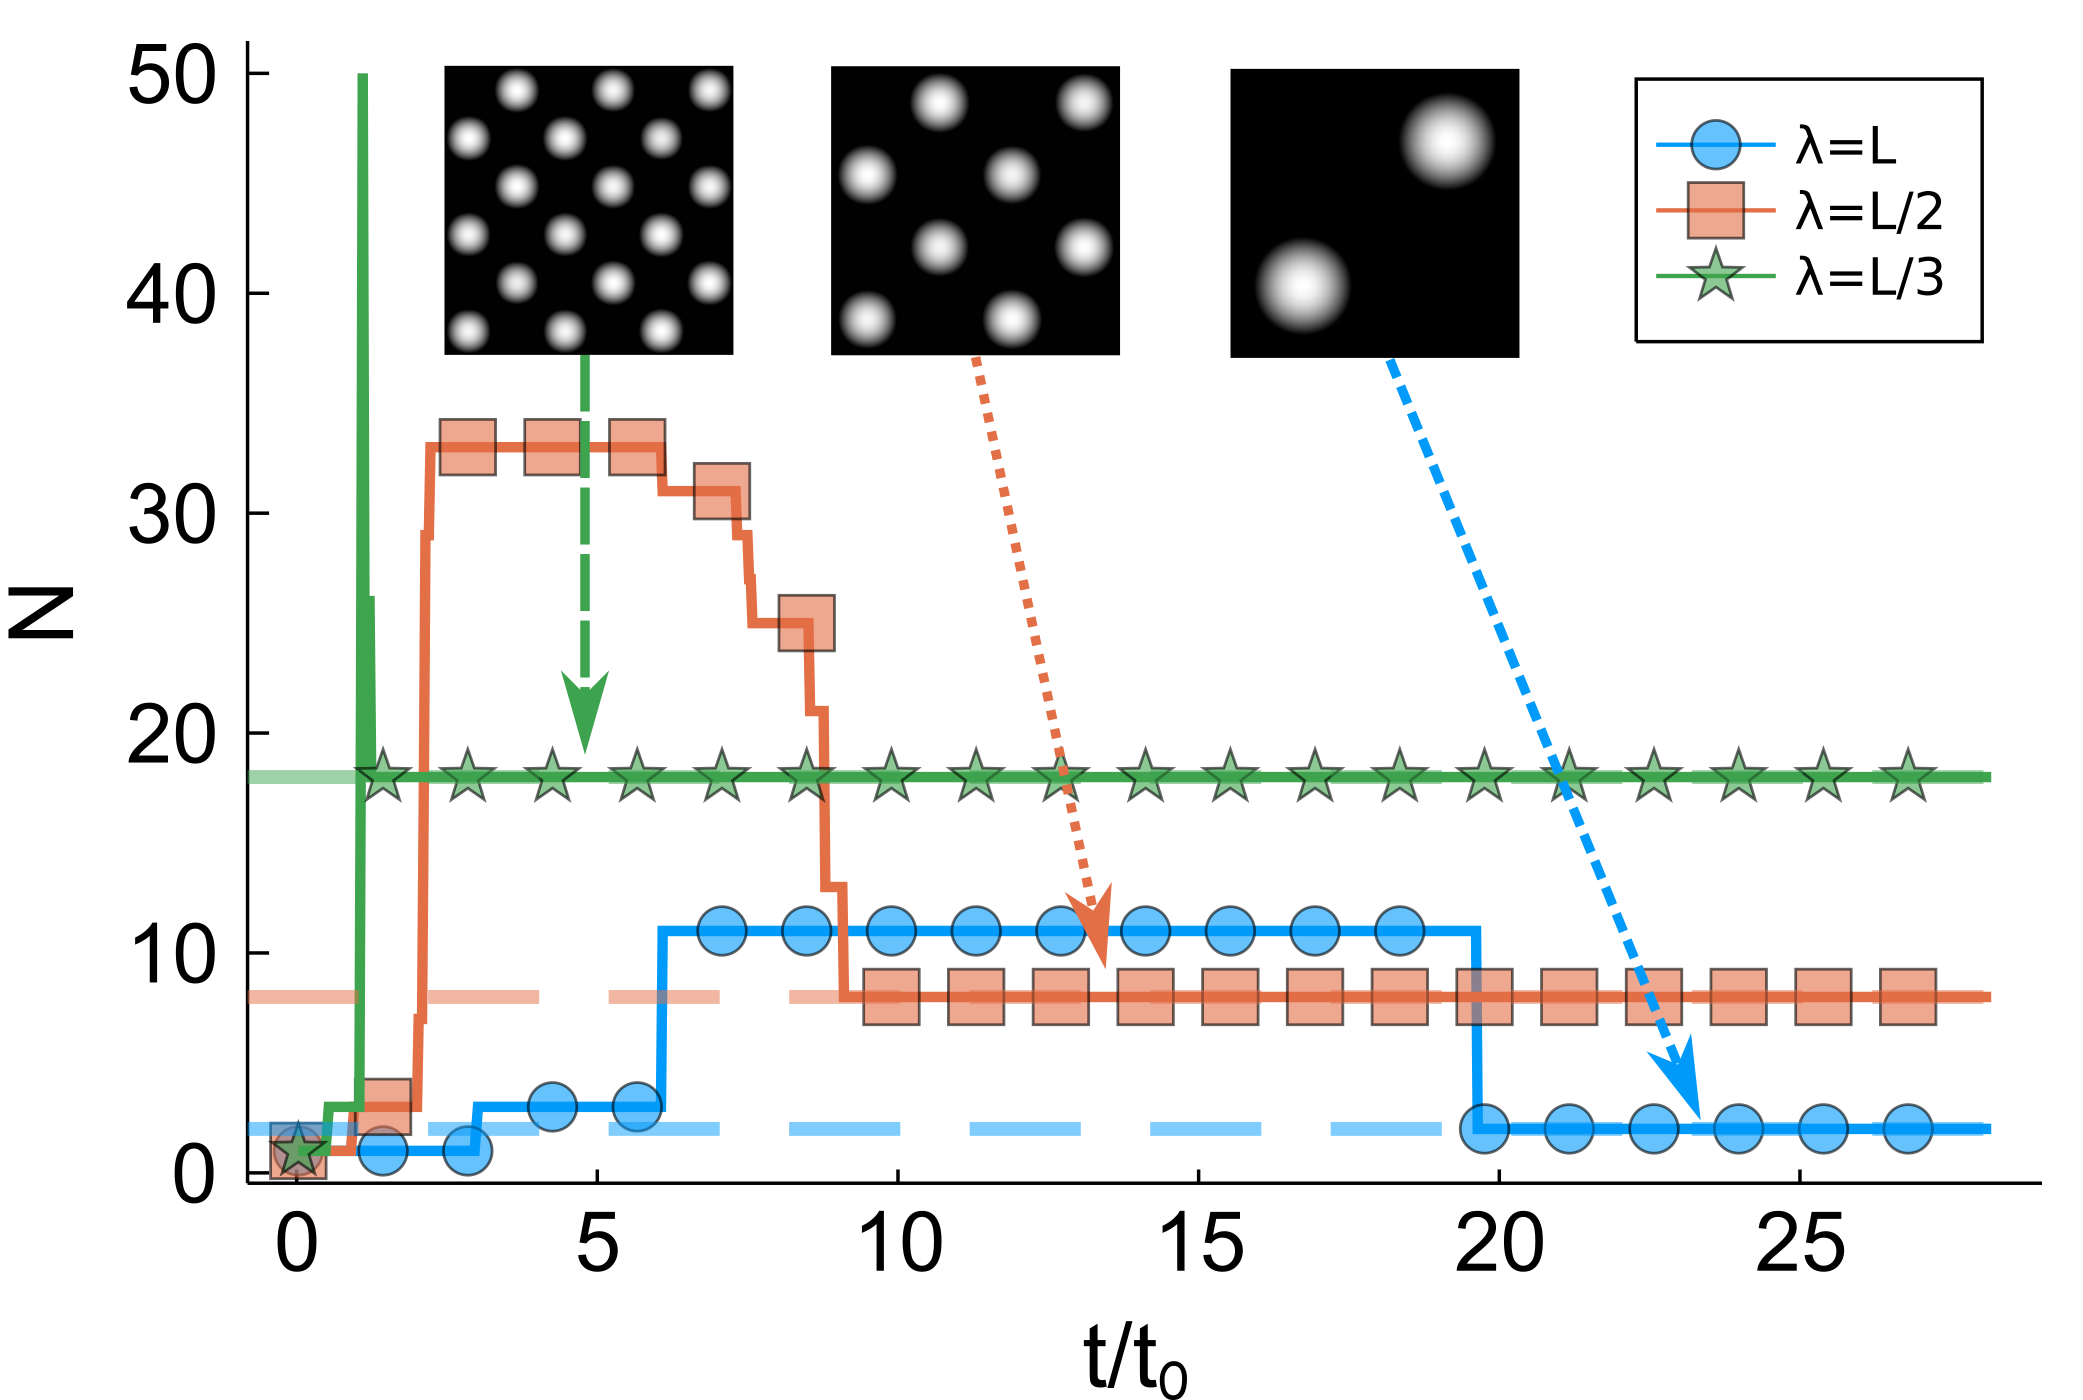
\includegraphics[width=0.48\textwidth]{Figures/Clusters_novel_sine_picutres.png}
    \caption{Connected component analysis of the film thickness for different wavelengths $\lambda$ on $\theta_1$ ($\theta_2$ matches qualitatively).
    On the x-axis we display the number of clusters while on the y-axis we show the time normalized by $t_0$.
    Different colors and symbols display different wavelengths $\lambda$.
    The three dashed lines indicate the number of minima the pattern offers.
    Above the data we show the stationary droplet state as a grayscale image of the film thickness $h(\mathbf{x},t_{\infty})$.}
    \label{fig:clusters_v0_sine}
\end{figure}
This is in fact a consistency check of our simulations.
We expect that in case of $v_{\theta} = 0$ all fluid accumulates in droplets inside the contact angle minima.
While there are only two minima for $\lambda = L$ there are eight and eighteen minima for $\lambda = L/2$ and $\lambda = L/3$ respectively.
This can be easily checked with a cluster analysis of the film thickness $h(\mathbf{x},t)$ which we shown in Fig.~\ref{fig:clusters_v0_sine}.
The height $h(\mathbf{x},t_{\infty})$ is displayed as grayscale images and is linked to stationary state.
Theoretically we expect therefor two, eight and eighteen clusters (droplets) which we mark with a vertical dashed line in the respective color.
These values are consistent with our simulations.
Interesting is the fact that the number of clusters converge faster for smaller wavelengths.
To some extend this is expected as the distance between contact angle minima is shorter for smaller wavelengths.

Another quantity that is easily accessible and helps to check the consistency of our simulations is the height of the droplets $h_d$.
Given that all the fluid is collected inside the droplets we can make an assumption of the droplets height based on its volume $V_d$  and contact angle $\theta_d$ 
\begin{equation}\label{eq:height_guess}
    h_d(V_d, \theta_d) = \left(\frac{3V_d(1-\cos(\theta_d)}{\pi(2+\cos(\theta_d))}\right)^{\frac{1}{3}},
\end{equation}
where we implicitly assume that all our droplets have a spherical cap shape.
Since our method does not allow $h=0$ we measure the droplets height as~\cite{PhysRevE.100.033313}
\begin{equation}\label{eq:delta_h_measure}
    \Delta h(t) = \max_{\mathbf{x}}\{h(\mathbf{x},t)\} - \min_{\mathbf{x}}\{h(\mathbf{x},t)\}.
\end{equation}
Counting the minima in $\theta(\mathbf{x})$ for the different wavelengths $\lambda$ allows to calculate the volume of a single droplet, see Fig.~\ref{fig:clusters_v0_sine}.
Since the film dewets regions of high contact angle values we can safely assume that $\theta_d < 20^{\circ}$.
\begin{figure}
    \centering
    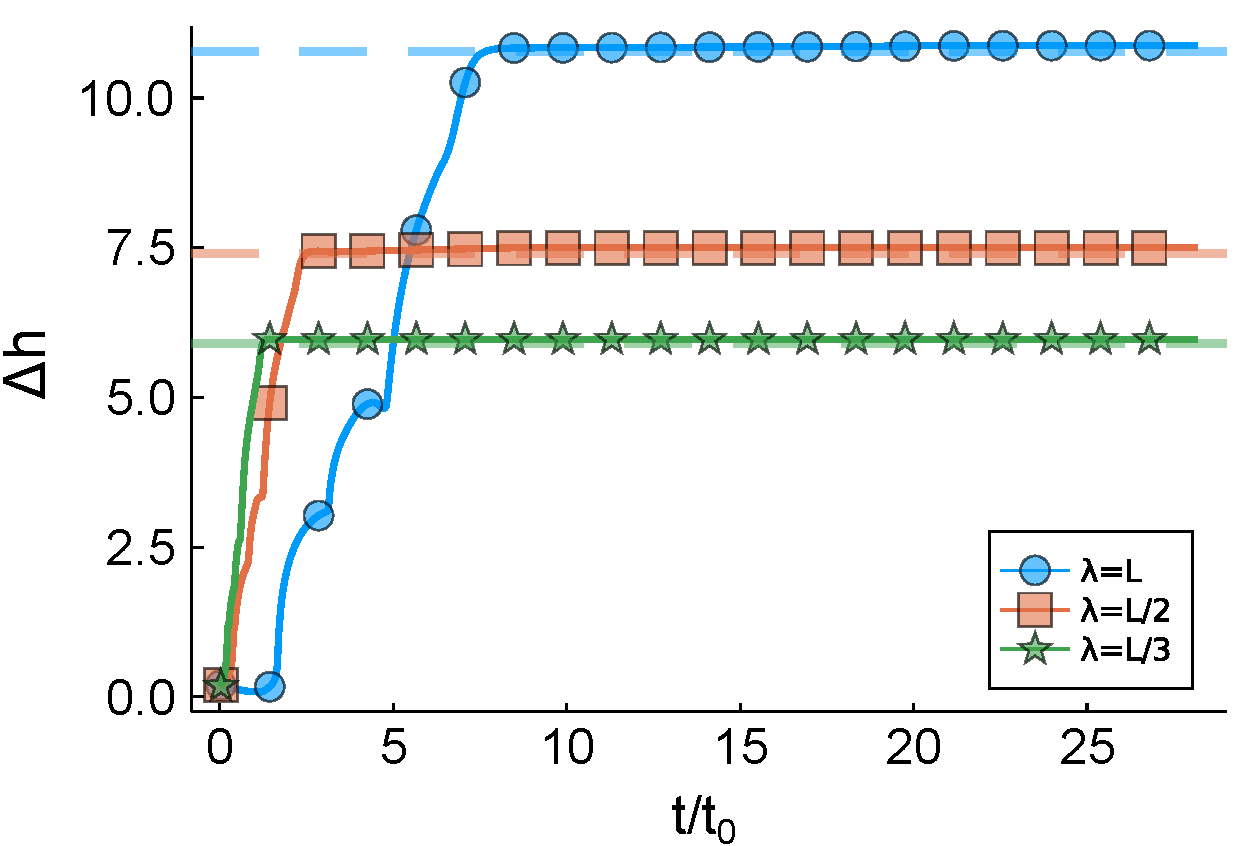
\includegraphics[width=0.48\textwidth]{Figures/delta_h_v0_sin_with_dash.pdf}
    \caption{Evolution of $\Delta h$ with time.
    Different symbols and colors represent different pattern wavelengths.
    Dashed lines indicate solutions to the cap height $h_d$ given the volume is split equally among the droplets, see Eq.~(\ref{eq:height_guess}).}
    \label{fig:deltah_v0_sine}
\end{figure}
Measuring the height of the droplets is done in Fig.~\ref{fig:deltah_v0_sine}, where $\Delta h$ is the maximal difference in film thickness which is equivalent to the droplet height $h_d$.
Focusing on the late time behaviour ($t > 10t_0$) we identify plateauing values. 
Since the pattern is a continuous functions, see Eq.~(\ref{eq:sinetheta}), we are left with some degree of freedom for the theoretical $\theta_d$ values. 
As a guide to the eye we introduce three dashed lines.
The dashed lines are calculated using Eq.~(\ref{eq:height_guess}) with $V_d = (V/2, V/8, V/18)$ and $\theta_d = (14^{\circ}, 16^{\circ}, 17^{\circ})$ for $\lambda=(L,L/2,L/3)$ respectively.
The values of $\theta_d$ are chosen to fit with the stationary droplet state of our simulations.
Thus we are fairly confident that our droplet states and thus the simulations capturing the correct physical state.

\subsection{Stability}\label{subsec:time_dep_theta}
\begin{table}[h!]
  \begin{center}
    \begin{tabular}{c|c|c|c}
      \textbf{Pattern} & \textbf{Wavelength} & \textbf{Velocity } & \textbf{Rupture time}\\
      $\theta(\mathbf{x})$ & $\lambda$ & $v/v_0 $ & $\tau_r/t_0$ \\
      \hline
      $\theta_1$ & L & 0 & 1.69\\
      $\theta_1$ & L & 0.1 & 1.72\\
      $\theta_1$ & L & 1 & 2.34\\
      $\theta_1$ & L & 10 & 2.25\\
      $\theta_1$ & L/2 & 0 & 0.39\\
      $\theta_1$ & L/2 & 0.1 & 0.39\\
      $\theta_1$ & L/2 & 1 & 0.59\\
      $\theta_1$ & L/2 & 10 & 0.68\\
      $\theta_1$ & L/3 & 0 & 0.23\\
      $\theta_1$ & L/3 & 0.1 & 0.23\\
      $\theta_1$ & L/3 & 1 & 0.25\\
      $\theta_1$ & L/3 & 10 & 0.45\\
      $\theta_2$ & L & 0 & 1.01\\
      $\theta_2$ & L & 0.1 & 1.18\\
      $\theta_2$ & L & 1 & 1.32\\
      $\theta_2$ & L & 10 & 1.38\\
      $\theta_2$ & L/2 & 0 & 0.48\\
      $\theta_2$ & L/2 & 0.1 & 0.48\\
      $\theta_2$ & L/2 & 1 & 0.7\\
      $\theta_2$ & L/2 & 10 & 0.76\\
      $\theta_2$ & L/3 & 0 & 0.39\\
      $\theta_2$ & L/3 & 0.1 & 0.42\\
      $\theta_2$ & L/3 & 1 & 0.68\\
      $\theta_2$ & L/3 & 10 & 0.76\\
    \end{tabular}
    \caption{Rupture time values for different pattern wavelengths $\lambda$ and different substrate velocities $v_{\theta}$.
    Due to sampling we have a systematic error of 0.03 in the rupture times $\tau_r$.}
    \label{tab:rup_times}
  \end{center}
\end{table}
Taking another look at Fig.~\ref{fig:deltah_v0_sine} reveals that the three wavelengths rupture at different times $\tau_r$.
The most important values for $\tau_r$ can be found in Tab.~\ref{tab:rup_times}.
We observe two features, first being that rupture time $\tau_r$ correlates with the wavelength $\lambda$.
Thus smaller values of $\lambda$ lead to an earlier rupture time.
Which can be explained with a mismatch of length scales.
There is a length scale set by Eq.~(\ref{eq:q0_and_t0}) ($\lambda_0 = 2\pi/q_0$) and one that we introduce with the substrates wavelength $\lambda$.
\begin{figure}
    \centering
    \includegraphics[width=0.48\textwidth]{Figures/RT_with_v10_inkscape.pdf}
    \caption{Distribution of rupture times $\tau_r$ normalized by $t_0$ for different pattern wavelengths $\lambda$.
    The bullets, stars correspond to data from our simulations with $v_{\theta} = 0, 10v_0$.
    Eq.~(\ref{fig:model_rt}) with $D=2$ is displayed by the blue line.
    }
    \label{fig:model_rt}
\end{figure}
Taking this into account we can model the rupture times for the stationary pattern with
\begin{equation}\label{eq:model_tr}
    \frac{\tau_r}{t_0} = \frac{1}{2\pi}\frac{L}{\lambda_0 i^D}\approx \xi\frac{\lambda}{\lambda_0},    
\end{equation}
where $i$ is the wavenumber of the substrates pattern ($\lambda = L/i$) and $D$ is the dimension, thus $D=2$.

Interestingly Eq.~(\ref{eq:model_tr}) is able to describe the data for $v_{\theta} = 0.1v_0$ as the difference of rupture times between these two simulations is negligible, see Tab.~\ref{tab:rup_times}.
Larger $v_{\theta}$ introduce a shift towards longer rupture times, therefore increasing the stability of the film.
Next we look into the affects of the pattern velocity on the structure formation after the first ruptures.

\subsection{Morphologies}\label{subsec:morphme}
Dewetting morphology is a rather broad topic~\cite{becker2003complex, RevModPhys.81.739, PhysRevLett.99.114503, craster2009dynamics, doi:10.1146/annurev-fluid-011212-140734, alizadeh_pahlavan_cueto-felgueroso_hosoi_mckinley_juanes_2018}, however we know that a simple patterned substrate will ultimately yield droplets in region of small contact angle and is likely to rupture in regions of high contact angle, as shown in Fig.~\ref{fig:handtheta}.
This is indeed what we observe for the simulation without pattern velocity ($v_{\theta} = 0$).
\begin{figure}
    \centering
    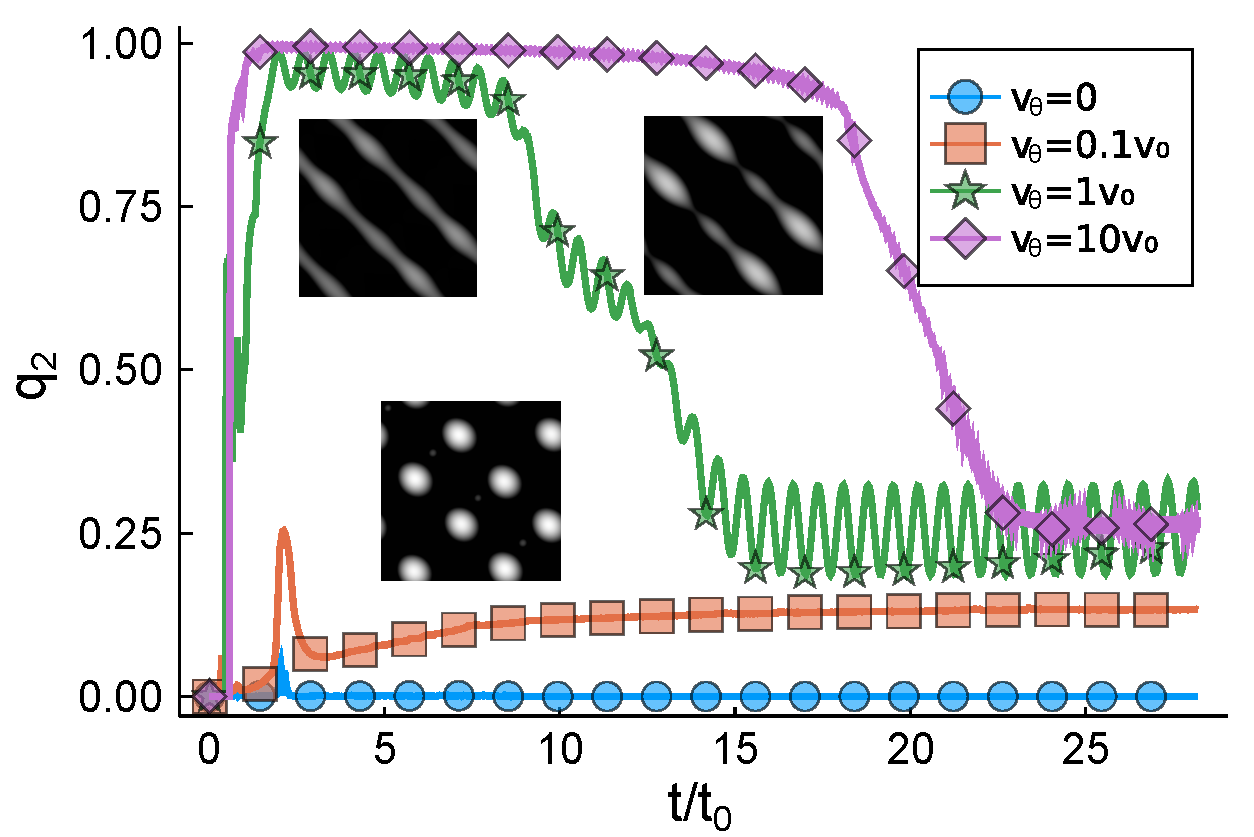
\includegraphics[width=0.48\textwidth]{Figures/q_2_different_v.pdf}
    \caption{Structure analysis of the pattern $\theta_1,~\lambda=L/2$ using the Minkowski structure metrics (MSM). 
    The dipole metric $q_2$ is plotted for different pattern velocities $v_{\theta}$, displayed with different colors and symbols.
    In grayscale we supply the film thickness that is associated with the $q_2$ values.
    }
    \label{fig:msm_q2}
\end{figure}
Increasing the pattern velocity $v_{\theta} > 0$ does affect the dewetting morphology quite substantially.
Having $v_{\theta} = 0.1 v_0$ we are still observing the formation of droplets, similar to $v_{\theta} = 0$ but instead of being stationary these droplets, depending on their mass, are transported with the contact angle minima.
A somewhat similar behaviour was recently described by Grawitter et al.~\cite{D0SM02082F} where they have used a boundary integral method to simulate a droplet on a moving wettability step.

If the pattern velocity is further increased $v_{\theta} > 0.1 v_0$ we observe a transition towards ligament or rivulet like structures.
These structures are aligned with the update direction of the contact angle field, see Eq.~(\ref{eq:theta_shift}). 
Thus if
\begin{equation*}
    \theta(x,y,t+T) = \theta(x-1, y, t),    
\end{equation*}
ligaments form in x direction.
These ligaments are sensitive to $\lambda$, or more precisely to the contact angle minima since they attract fluid.
To classify the morphological differences in respect to $v_{\theta}$ we make use of the software \textbf{papaya2}~\cite{Schaller2020}.

We use the film thickness as input and compute different morphological metrics.
Among the most interesting ones are the Minkowski structure metrics (MSM) $q_s$.
They can be calculated using~\cite{doi:10.1063/1.4774084}
\begin{equation}
    q_s(K) = \frac{|\psi_s(K)|}{\psi_0(K)}, 
\end{equation}
where $K$ is the body to we extract morphological information from and $\psi_s$ are the irreducible Minskovski tensors (IMT)
\begin{equation}
    \psi_s(K) = \int_{0}^{2\pi}e^{is\phi}\rho_K(\phi) \dd\phi = \sum_{k=-\infty}^{\infty} L_k e^{is\phi_k},
\end{equation}
with $L_k$ being the set of normal vectors of the body $K$.
Within the various $q_s$ we are particularly interested in the dipole one $q_2$. 
With $q_2$ we can clearly distinguish between a droplet and a ligament structure, as we expect a much larger $q_2$ value for the ligament state which is what we see in Fig.~\ref{fig:msm_q2}.
Our simulations with $\lambda = L/2$ show a clear difference between $v_{\theta} \leq 0.1v_0$ and $v_{\theta}>0.1v_0$  in $q_2$.
Interestingly the $q_2$ values for $v_{\theta} = 0.1v_0$ are always larger than those of $v_{\theta} = 0$.
The difference is due to the distortion of the droplets surface area as it is transported with the pattern.

Moving the contact angle field faster creates metastable ligament states.
Metastable because this ligaments will eventually break and separate into droplets, as indicated by the dip in $q_2$ for $v_{\theta} = 1, 10 v_0$ in Fig.~\ref{fig:msm_q2}.
Nevertheless their formation in the first place can be explained with a few relative simple assumptions.

This problem is associated with two time scales, first being $t_0(\theta)$ the time scale of the dewetting thin film, see Eq.~(\ref{eq:q0_and_t0}).
After the rupture we identify another time scale, the capillary time scale $\tau_{\text{Ca}}$ that drives the rims away from the holes~\cite{Edwardse1600183},
\begin{equation}\label{eq:cap_time}
    \tau_{\text{Ca}} = \frac{9\mu l_0}{\gamma \theta^3(\mathbf{x})},
\end{equation}
where  $l_0$ is a characteristic length scale of the problem, we use $\lambda/2$ as two rims can travel at most $\lambda/2$ before they merge.
Knowing this time scales allows us to introduce characteristic velocities.
One of these two is $v_0$ which is given by Eq.~(\ref{eq:normvel}) and used to normalize $v_{\theta}$.
The other one is set by $\tau_{\text{Ca}}$ and reads
\begin{equation}\label{eq:cap_speed}
    U_{Ca} =\frac{l_0}{\tau_{\text{Ca}}} = \frac{\gamma}{9\mu} \theta^3(\mathbf{x}), 
\end{equation}
where $U_{\text{Ca}}$ is the capillary speed.
The argument is as follows, if $U_{\text{Ca}}$ is large as compared to $v_{\theta}$ than the film retraction is faster than the transport due to the contact angle field and thus droplets from.
Which explains the cases of $v_{\theta} = 0, 0.1v_0$.
On the other hand if $v_{\theta}$ is larger than $U_{\text{Ca}}$ than the retracting film has to little time to create stable droplets and ends up in the metastable ligament state.
Taking a look at our simulations with $v_{\theta} = 1, 10v_0$ we clearly observe ligament states.

In fact the ratio 
\begin{equation}\label{eq:vel_ratio}
    \Gamma = \frac{v_{\theta}}{U_{\text{Ca}}} = \frac{3\lambda \chi h_0^3 q_0^4}{\Theta^3}, 
\end{equation}
where $\Theta = max(\theta(\mathbf{x}))$ and $v_{\theta} = \chi v_0$, allows to classify the dewetting morphology on a time and space dependent substrate pattern as
\begin{equation}\label{eq:classify}
    \Gamma~\begin{cases}
    < 1\qquad ... \text{droplets} \\
    > 1\qquad ... \text{ligaments} 
    \end{cases}.
\end{equation}
This explains in fact what we observe and holds true independent of the wettability gradient, i.e. $\theta_1, \theta_2$.

Therefore by varying either $\chi$ or $\lambda$ for a fixed $\Theta$ one can change the intermediate dewetting morphology according to the equation above.
Interestingly but not surprising is the fact that the fluid transport is larger for $\Gamma > 1$ than for $\Gamma < 1$.

\section{Summary and Conclusions}\label{sec:sum_conclu}
To summarize, we have shown numerical simulations of a dewetting thin film on a patterned substrate.
Generating baseline experiments with time independent patterns of different wavelengths, we than move to a time and spatial varying contact angle field $\theta(\mathbf{x},t)$.

In the next step we define a characteristic pattern velocity $v_0$ which simply is the patterns wavelength $\lambda$ over a characteristic time $t_0$, see Eqs.~(\ref{eq:q0_and_t0}, \ref{eq:normvel}).
Experiments with increasing pattern velocity $v_{\theta} = \chi v_0$ with $\chi\in\{0,10\}$ show a pronounced change in dewetting morphology from well defined droplets to ligaments.
With the single balance between pattern velocity $v_{\theta}$ and capillary velocity $U_{\text{Ca}}$ we can identify a parameter that separates the two morphological regimes.

An outlook to this work is to study the transition from ligaments to droplets in a more detailed manner.
Looking at the edges $\Gamma =1$ with more suitable tools like e.g. bifurcation diagramms will likely be subject to future work.
But also the update scheme of the contact angle field allows for many applications.
Among them is the avenue of switchable substrates, where e.g. switching of $\theta(\mathbf{x})$ due to a light source is in the scope of this method.


\begin{acknowledgements}
The authors acknowledge financial support by the Deutsche Forschungsgemeinschaft (DFG) within the priority program SPP2171 ``Dynamic Wetting of Flexible, Adaptive, and Switchable Substrates'', project HA-4382/11.
\end{acknowledgements}

%\appendix
%\section{}\label{app:one}

\bibliography{Ref}

\end{document}